\documentclass[10pt,a4paper]{article}
\usepackage[french]{babel}
\usepackage[utf8x]{inputenc}
\usepackage{ucs}

\usepackage{amsmath}
\usepackage{amsfonts}
\usepackage{amssymb}

\author{LAFON Sylvain, MAINGRET François et LEVASSEUR Thomas}
\title{Projet "Bob-Project"}
\begin{document}
\maketitle
\tableofcontents
\newpage
	\part{Introduction}
		Le bricolage et le jardinage etants à la mode des derniers temps, le site Brico-Bob vise à proposer à des utilisateurs de profils variés, aussi bien
la ménagère que le retraité ou que les jeunes couples, du matériel à la vente ou à la location.
Ce site étant de nature commerciale, il se doit d'etre visuellement attractif et d'etre ergonomique. La présentation des produits devra etre simple, claire, et 
bien organisée, l'utilisateur devra pouvoir trouver un produit le plus rapidement possible afin qu'il ne se lasse pas du site et qu'il achète le plus de prosuits
possible ( De plus, il existera une fonction pour rechercher un produit selon differents critères. De la publicité sur certaines pages du site pourra influencer
le client.
Chaque utilisateur du site devra s'inscrire en fournissant un login et un mot de passe pour  faire ses achats, ses informations personnelles ( nom, adresse... )
ne seront demandées que lors de la validation de la commande ). Chaque membre du site pourra poster des avis, et noter les differents produits, ainsi que poser
des questions techniques.
Enfin, l'administrateur du site pourra gerer simplement, depuis une fenetre speciale, le contenu du magasin, et les membres.

	
	\part{Bob-Project}
		\section{Objectif}
			L'objectif de ce projet était de réaliser un site web pour un magasin de bricolage, Brico-Bob.  Ce site devra gérer plusieurs aspects : une partie privée et une partie publique. La partie publique sera accessible a n'importe qui, et comprendra, entre autres, la possibilités de visionner des produits, d'en rechercher, de commenter un produit. La partie privée sera réservée aux administrateurs du site et comprendra un panneau permettant de gérer tout le contenu du site, des produits, images, catégories...  
		\section{Objectifs du site}
		L'objectif de notre site est de proposer à la vente comme à la location des articles de bricolage pour le grand public.  Le site devra donc être assez ergonomique et  attrayant visuellement afin de ne pas repousser les visiteurs.\\
		
Voila les points importants sur lesquels sur lesquels nous avons fait attention :
			\begin{itemize}
\item Un temps de chargement des pages optimisé. En effet On estime le seuil d'acceptation de chargement d'un site à deux secondes (selon plus de 47\%  des internautes sondés).  Au delà, vous commencez à perdre des visiteurs. ( source : Marketing Management par  P. Kotler ).\\

\item Proposer une description des produits assez détaillée : si le client ne trouve 	pas 	assez d'informations sur un produit sur notre site, il ira chercher ces 	informations chez un concurrent, et a moins que notre prix soit 	significativement plus bas, il y a de grandes chances qu'il achète chez ce 	concurrent.\\

	
\item Il faudra utiliser le plus de termes simples a comprendre par l'utilisateur plutôt 	que des termes techniques barbares.  Notre site permet donc d'écrire de 	longues description, mais cette responsabilité incombe plutôt à la société Brico-	Bob.\\

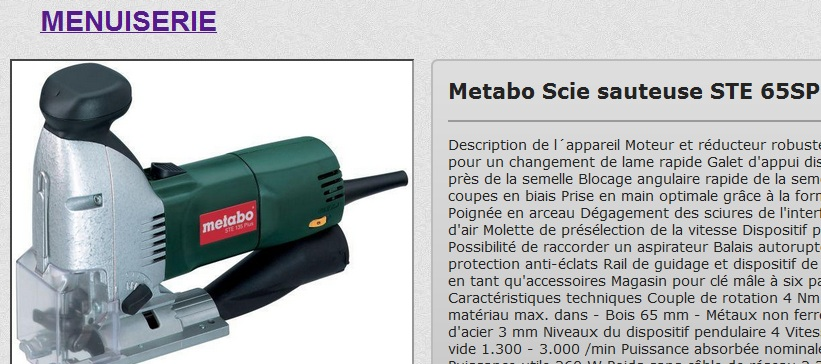
\includegraphics[scale=0.5]{demofichepro.jpg}

\item Donner des informations sur la société et sur le service client, ainsi que les 	administrateurs du site. Le client veut savoir a qui il a affaire et sera plus enclin 	à acheter si il sait qu'il peut contacter quelqu'un ensuite. Le client sera mis en 	confiance, ce qui est vraiment important lorsque son argent est en jeu.\\
	Ces informations seront donc accessibles depuis n'importe quelle page du site 	grâce au menu :\\

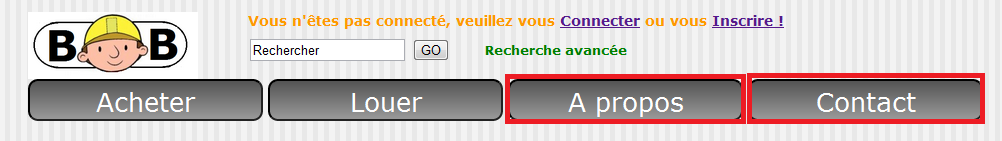
\includegraphics[scale=0.5]{menu.jpg}

\item Ne pas trop s'introduire dans la vie privée du client : nous n'avons demandé 	au client que des informations non personnelles lors de son inscription :  son 	pseudo et un mot de passe. Il n'as pas besoin de donner son nom ni son 	adresse tant qu'il ne valide pas une commande. Cela lui permettra de ne pas se  	sentir "tracké" et de visiter librement le site.\\

\item Un moteur de recherche bien réalisé. Si le client sait exactement ce qu'il veut 	lorsqu'il va sur le site, il ira chercher le nom du produit qu'il a en tête dans la 	barre de recherche. Si le moteur de recherche n'est pas bien conçu, il risque de 	penser que nous n'avons pas le produit qu'il cherche et il ira donc voir ailleurs. 	Si il n'a qu'une idée très vague, il y a alors des chances qu'il se tourne vers le 	moteur de recherche avancée. Cela nous permettra de cerner ses critères de 	prix par exemple.\\

\item Mettre en évidence le produit en mettant une image assez grande : trop de site proposent encore des images ridiculement petites, ce qui peut décourager le client d'acheter, car il ne peut pas bien voir le produit et peut même penser qu'il y a des risques de "tromperie" sur la marchandise.\\

\item Une navigation aisée, c'est à dire des catégories bien organisées. Bien que notre site permette d'afficher à la fois des produits et des catégories sur une même page, cela sera à éviter dans le cas général. Enfin, il faudra veiller à ne pas créer de catégories vides, qui prendrait de la place pour rien et serait une source de  frustration pour le client ( quoi de plus désagréable que de trouver une catégorie qui correspond parfaitement à ce que l'on recherche et se rendre compte qu'elle est vide )\\

\item Mettre l'accent sur les produits : le but d'un site de e commerce est de vendre, et nous avons donc fait attention de mettre l'accent sur les produits. Le design est assez sobre, et les autres éléments du site 	n'empiètent as sur les produits. Il y a également sur la page d'accueil des "coups de cœur" permettant de stimuler un achat imprévu chez le client.


\end{itemize}
		\section{Logique et Organisation}
			%Logique et Organisation
\subsection{Fichiers}
	\subsubsection{header.php}
	Ce fichier va insérer la bibliothèque Smarty et les déclarations de classes, puis il va déclarer des constantes et crée quelques fonctions.
	
\subsubsection{index.php}
	Ce fichier va tout d'abord appeller header.php puis va créer l'objet Bob et smarty.\\
	Il va ensuite analyser la requete pour savoir quel template il va appeller pour fabriquer la page et va effectuer les actions qu'on lui demande de faire.\\
	Il va ensuite passer à Smarty plusieurs variables puis générer la page.

\subsubsection{les fichiers de /classes et de /Smarty}
	Ces fichiers contiennent les classes qui contiennent les infos de la base de données et qui la manipule.
	
\subsubsection{les fichiers de /templates}
	Ils permettent d'afficher une page en utilisant les variables qu'on lui prete, il y a deux style de templates : 	
\begin{itemize}
	\item les fichiers modèle : ils se situent dans /templates/modele
	\begin{itemize}
		\item main.tpl : Contient ce que toute page va contenir, il va appeller les autres fichiers templates de modèle
		\item menu.tpl : Contient le menu du site
		\item entete.tpl  : Contient les informations sur la page ($<head>$)
		\item espace\_membre.tpl : Contient l'espace membre\\
	\end{itemize}
					
	\item le fichier appelé pour la page : ils se situent dans /templates.\\
	Il y en a un par page
	\end{itemize}
	
\subsubsection{les fichiers de /css}
	Ils permettent de coder le design du site, ils se situent dans /css. Ces fichiers sont séparés en plusieurs fichiers. On préférera en mettre un général puis un par page.
\newpage
\subsubsection{En somme}
Seul index.php permet de générer une page, il va commencer par appeller toutes les ressources à l'aide de header.php (qui inclut les classes de /classes et /Smarty), il va ensuite regarder le type de la requete :
\begin{itemize}
\item Est-ce pour le panneau d'admin, une image, une information ?
\item Est-ce une page ou une action que l'on nous demande ?
\end{itemize}

En fonction de cela nous allons faire telle ou telle action (méthodes de la classe Bob) puis choisir tel ou tel template à appeller.\\

Une fois l'action faite et le template choisi, Smarty (l'objet) va prendre certaines variables (contenues dans Bob, ses attributs ainsi qu'un eventuel message) puis va utiliser le template pour générer une page.\\

Le template appellé est une extension du template modèle templates/modele/main.tpl (divisé en plusieurs templates modèles),
cela permet de garder une meme forme pour chaque page : seul le contenu, certains scripts sera modifié d'une page à l'autre !\\

La page html ainsi générée fera appel à certaines feuilles de design de /css et à certains scripts /js
	\newpage
\subsection{Catégories}
	%Catégories
Comme nous l'avions dit dans les objectifs du Site, la navigation se fait par un système de catégories qui peuvent contenir d'autres catégories et d'autres produits.\\
(c'est à l'administrateur à faire attention à ne pas de creer de catégories vides, pour des raisons d'ergonomie, il est aussi conseillé d'éviter de mettre catégories et produits ensemble)\\

Tout ceci se résume à un simple schéma :\\

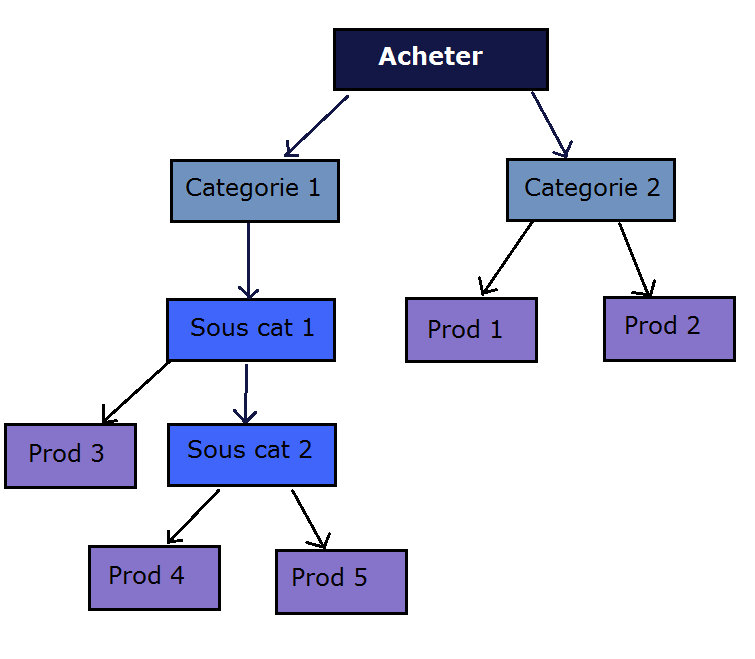
\includegraphics[scale=0.5]{Images/arbocatego.png}
\newpage
	\newpage
\subsection{Pages}
	% Pages
Plutot que de parler une à une de chauqe page 'logique' du site, voici un schèma plus explicite :\\

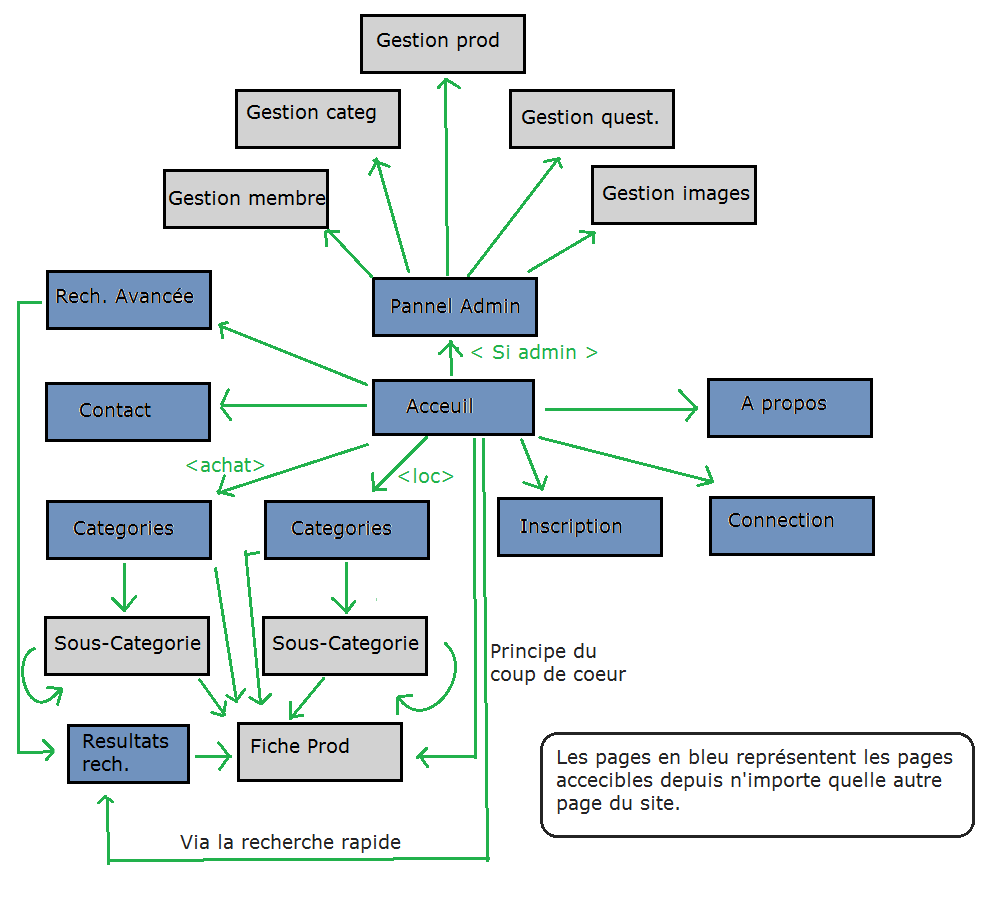
\includegraphics[scale=0.5]{Images/arbo.png}



	\newpage
			
		\section{Architecture des pages}
			\input{archi.tex}
		\section{Technologies utilisées}
			% Technologies utilisées

\subsection{Support du code}
	% Support du code
Pour le projet nous avons utilisé plusieurs supports :\\
\begin{description}
	\item[Github :] Il s'agit d'un système de partage de projets gratuit -si on accepte de les mettre open-source- très pratique.
	\item[Notepad++ :] Il s'agit de notre éditeur de texte favori, nous l'avons tous utilisé
	\item[Wamp/Lampp :] Il s'agit d'un émulateur de serveur Apache/MySql/Php pour pouvoir tester le site en local.
		\begin{description}
			\item[Apache :] Il émule le serveur en lui meme, il contient notemment une interface "phpMyAdmin" et "Wamp" (pour les différents projets)
			\item[MySql :] Il émule la base de données
			\item[Php :] Le programme qui, suivant la requete, interpretera la bonne page php.
		\end{description}
	\item[The GIMP :] C'est un outil pour manipuler les images très puissant : beaucoup d'éléments ont été réalisées grace à lui.
\end{description}

\subsection{Les langages de programmation}
	% Langages

Nous avons utilisé, comme pour la plupart des sites, les langages :
\begin{description}
	\item[HTML :] Il défini les éléments de la page dans les templates	
	\item[CSS :] Il gère le design du site, nous avons séparé ses fichiers en plusieurs parties (Au départ il s'incluait tous, mais nous avons fait en sorte que Smarty n'appelle que ceux qui nous importe)
	\item[PHP :] Il permet de creer la page HTML suivant la requête qu'on lui donne.	
	\item[SQL :] Il est utilisé par Php pour manipuler la base de données, laquelle contient tous les éléments du site, lesquels sont stockés au chargement de la page dans des objets (Php)	
	\item[JavaScript :] Il permet de faire "Bouger la page" chez le client, sans avoir besoin d'envoyer de requête Php.\\
	Cela permet, par exemple, de faire un premier contrôle local des données que le client veut envoyer mais cela permet aussi, de rendre certains elements plus ergonomiques, par exemple pour la notation des produits.
\end{description}
	
\subsection{Les bibliothèques utilisées}
	Nous avons utilisé deux bibliothèques :
\begin{description}
	\item[AJAX :] Exploité par le JavaScript, elle permet de récuperer une autre page et de traiter ces données alors que la page ayant appelé AJAX est encore active.\\
Elle permet, par exemple, alors que la page d'inscription est affichée, de demander au serveur si tel ou tel pseudo est utilisé ou non.

	\item[Smarty :] C'est le moteur de templates utilisé, il permet de séparer traitement des données et mise en page : Le code Php qui l'appelle va commencer par analyser la requête, et suivant son analyse va appeler tel ou tel template en lui 'passant' des variables qu'il pourra alors utiliser pour l'affichage.
\end{description}

		\section{Base de données}
			% Base de données 
Elle contient toutes les infos du site, notemment :
\begin{itemize}
	\item Les membres
	\item Les catégories
	\item Les produits
	\item Les commentaires
	\item Et meme les images !
\end{itemize}

Voici un schéma relationnel de notre base (généré à l'aide de "MySql Workbench")\\

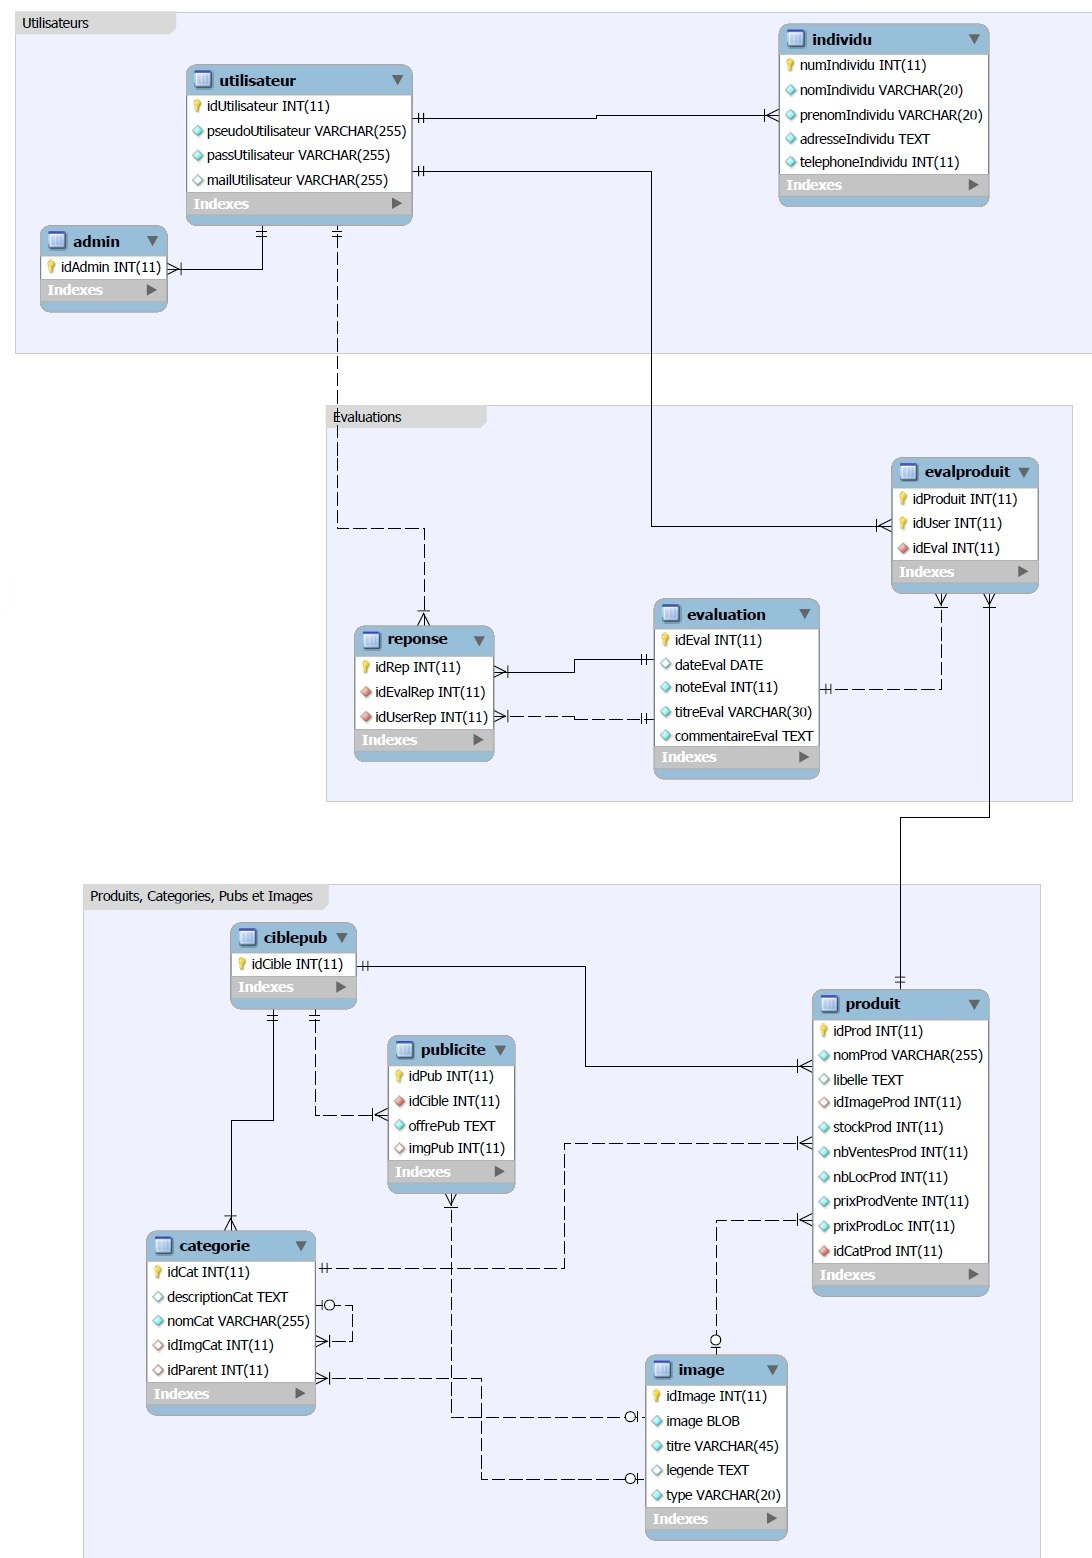
\includegraphics[scale=0.5]{Images/dbob.jpg}	
		\section{Les sessions}
			% Les sessions

Nous n'avons pas surutilisé les sessions : Nous ne les avons utilisé en fait, que pour la connexion :\\

Si l'internaute est connecté, alors une session contenant le booleen 'connecte' et les informations sur lui (dont l'id)
\begin{description}
	\item[Avantages :] Permet de détruire 'connecte' pour déconnecter l'utilisateur sans avoir à recharger la page.
	\item[Inconvénient :] N'utilisant pas QUE l'id mais surtout les autres informations que nous avons entré à la connexion du membre, et bien si des modifications sont faites, l'utilisateur ne le vera qu'à sa prochaine connexion. (Il suffira d'utiliser l'id pour changer cela)
\end{description}

Nous pourrions utiliser les sessions pour un éventuel captcha lors de l'inscription.
		\section{Portabilité}
			% Portabilité
\subsection{Différents navigateurs}

	Notre application est fonctionnelle sur les versions récentes de Google chrome, internet explorer et Firefox. Le site fonctionne également sur des versions un peu plus anciennes, par exemple sur IE6. ( Nous n'avons pas utilisé de HTML5 ). La différence est que les navigateurs un peu anciens ne reconnaissent pas certaines propriétés CSS3 utilisées par exemple box-shadow ou les effets de dégradé. Cependant, nous avons fait en sorte que l'affichage reste "décent", même si le site sera quelque peu moins beau.

\subsection{Javascript}

	Si le visiteur désactive le Javascript, le site ne sera pas moins fonctionnel, seulement, certains menus seront légèrement moins intuitifs et beaux. Il devra par exemple re-remplir tout le formulaire d'inscription si il fait une erreur mais cela ne changera rien au fait que l'inscription se déroulera normalement.
	
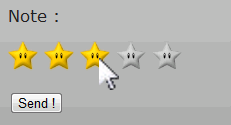
\includegraphics[scale=1]{Images/exemplejs.png}
		\section{Flexibilité} % Résistance aux changements
			% Flexibilite
\subsection{Changement du design du site}
	Si le client veut changer le design du site, il suffira de changer les fichiers .css ainsi que les images dans le dossier img. Par exemple pour changer les couleurs, la commande "remplacer tout" de notepad++ permettrait de changer les codes hexa assez rapidement.

\subsection{Type de matériel}
	Si le client veut que son site soit conçu pour une taille d'écran bien précise, il faudrait alors changer la taille de la page dans les fichiers ,css ainsi que d'agrandir certaines boites grâce a la propriété CSS width.

\subsection{Changement du contenu}
	Notre site est adapté au cas ou on voudrait changer son contenu. Si le client ne souhaite plus vendre de produits de bricolage, mais de l'électroménager.
Il suffirait de changer les noms des produits, catégories et de changer quelques images pour coller avec le nouveau thème du site.	

		
	\part{Conclusion}
		\input{conclusion.tex}
\end{document}